\documentclass{article}
\usepackage[utf8]{inputenc}
\usepackage{graphicx}
\usepackage{setspace} % Added for line spacing control
\usepackage[margin=2.5cm]{geometry}
\usepackage{hyperref}
\usepackage{polski}
\usepackage{amsmath}
\usepackage{subcaption}
\usepackage{listings}
\usepackage{xcolor}  % For coloring your code


\captionsetup{skip=0cm}  % Adjust the space between the figure and caption

% Define dark theme style for code
\lstdefinestyle{darkcolab}{
    backgroundcolor=\color{black},   % Dark background
    commentstyle=\color{green},      % Green for comments
    keywordstyle=\color{cyan},       % Cyan for keywords (like Colab)
    numberstyle=\tiny\color{gray},   % Line numbers in gray
    stringstyle=\color{orange},      % Strings in orange
    basicstyle=\ttfamily\footnotesize\color{white},   % Code in white
    breaklines=true,                 % Automatic line breaking
    captionpos=b,                    % Caption below the code
    numbers=left,                    % Line numbers on the left
    numbersep=8pt,                   % Space between numbers and code
    frame=single,                    % Frame around the code
    tabsize=4,                       % Tab size
    showstringspaces=false,          % Don't show spaces
    rulecolor=\color{gray},          % Frame color in gray
    morekeywords={self, np, plt},    % Add additional keywords
}

\lstset{style=darkcolab}

\title{\textbf{Analiza i klasteryzacja zbioru koktajli}}
\author{Aleksandr Shestakov \\
        nr index 272657 \\
        Politechnika Wrocławska \\
        Wydział W4N \\}
\date{27 October 2024}

\begin{document}

\maketitle

\vspace{100cm}

\tableofcontents

\section{Cele projektu}
Celem projektu jest przeprowadzenie preprocessingu, augmentacji i EDA podanego zbioru koktajli oraz klasteryzacji tego zbioru.

\section{Inital data analysis}
Startowy zbiór danych zawiera 134 wiersza i 11 kolumn, co odpowiada 134 koktajlam.
\subsection{Cechy}
Startowy zbiór zawiera kolejne cechy:
\begin{itemize}
    \item id
    \item name - nazwa koktajlu
    \item category - kategoria (Ordinary Drink, Cocktail lub Punch / Party Drink)
    \item glass - szklanka do serwowania koktajla, spis zostanie podany później
    \item tags
    \item instructions - instrkucja do przyrządzenia koktajla
    \item imageUrl
    \item alcoholic - czy koktajl jest alkoholowy
    \item createdAt
    \item updatedAt
    \item ingredients - lista słowników ze składnikami koktajla
\end{itemize}


\subsection{Wyniki IDA}:
\begin{itemize}
    \item Wszystkie koktajli okazały się alkoholowymi
    \item 99 koktajli nie mają danych o ich tag'ach
    \item createdAt i updatedAt - daty który nie różnią się między sobą i jak podejrzę są momentami w których dane zostali wyciągnięty z TheCokctailDB 
    \item Duplikatów koktajli nie okazało się - wszystkie wierszy dotyczą unikatowych koktajli
\end{itemize}
Kolumny id, imageUrl, alcoholic, createdAt, updatedAt - zostały wyrzucone jako niepotrzebne do analizy.

Ostateczny wynik po tym etapie:
\begin{figure}[htbp]
\centering
    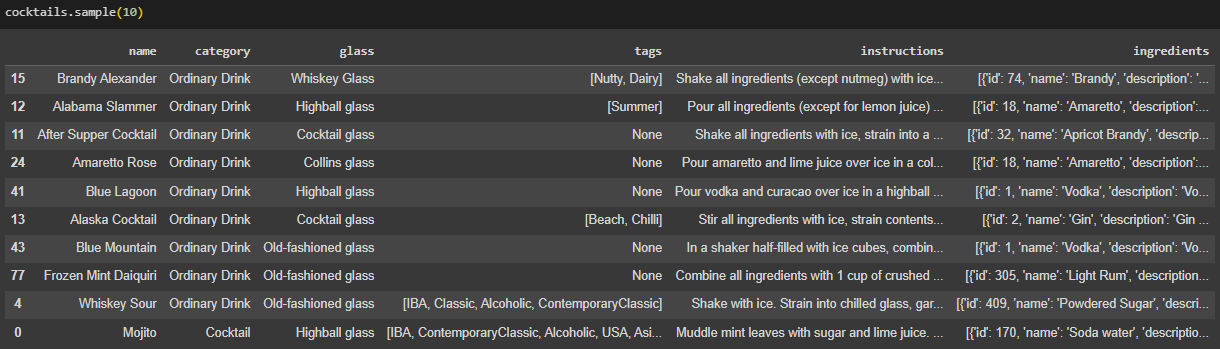
\includegraphics[width=1\linewidth]{cocktails_1.png}
    \caption{Tabela koktajli}
\end{figure}


\clearpage

\section{Preprocesing i augmentacja}
\subsection{Tabela składników}
W tym punkcie zostanie opracowana tabela wszystkich składników spotykanych we wszystkich koktajlach zbioru.
Tabela od razu po wyciągnięciu danych o składnikach z tabeli koktajlów:
\begin{figure}[h]
\centering
    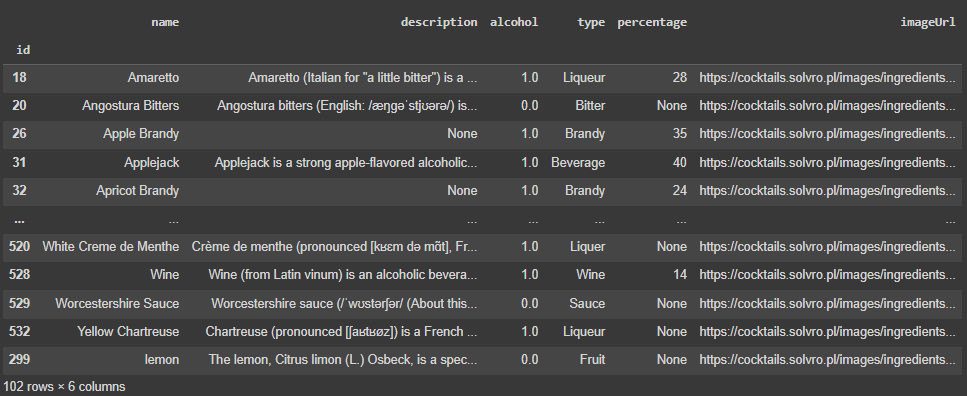
\includegraphics[width=1\linewidth]{ingredients_1.png}
    \caption{Tabela składników}
\end{figure}



\subsubsection{Typy składników}
Widzimy że tabela zawiera 102 składniki i 6 kolumn dla ich opisania
Dalej widać że w tabeli jest kolumna \textbf{type}, w której widzimy podobne znaczenia:
\begin{itemize}
    \item Liqueur i Liquer
    \item Bitter i Bitters
    \item A oznaczony jako Beverage Applejack, tak naprawdę jest typu Brandy
\end{itemize}


\begin{figure}[htbp]
\centering
    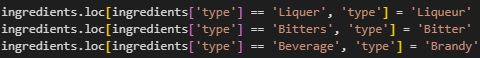
\includegraphics[width=0.6\linewidth]{ingredients_2.png}
    \caption{Typy składników}
\end{figure}

Dalej uogólnimy type składników dla dalszej analizy za pomocą podanego mapper'a
\begin{lstlisting}[language=Python]
# Creating less specific types of ingridients for future analysis
def ingredient_type_mapper(ingr_type):
  ingredient_mapping = {
      'Liqueur': 'Alcoholic',
      'Bitter': 'Alcoholic',
      'Brandy': 'Alcoholic',
      'Rum': 'Alcoholic',
      'Whiskey': 'Alcoholic',
      'Whisky': 'Alcoholic',
      'Spirit': 'Alcoholic',
      'Wine': 'Alcoholic',
      'Fortified Wine': 'Alcoholic',
      'Gin': 'Alcoholic',
      'Vodka': 'Alcoholic',
      'Water': 'Non-Alcoholic',
      'Soft Drink': 'Non-Alcoholic',
      'Juice': 'Non-Alcoholic',
      'Syrup': 'Non-Alcoholic',
      'Soda': 'Non-Alcoholic',
      'Tea': 'Non-Alcoholic',
      'Cream': 'Toppings',
      'Sauce': 'Toppings',
      'Mineral': 'Toppings',
      'Fruit': 'Fruit',
      'Flower': 'Decoration'
  }

  return ingredient_mapping.get(ingr_type, pd.NA)

ingredients['generalized_type'] = ingredients['type'].apply(ingredient_type_mapper)
\end{lstlisting}

Takie podejście popełnia błędy w raziee jeżeli alkoholowy składnik nie ma typu, ale później to będzie naprawione.



\subsubsection{Mocność alkolowych składników}
Jeżeli sprawdzić jakie typy alkoholi mają choćby jeden wpis z danymi o mocności, to można zauważyć ża takich typów składników jest 8, a wszystkich typów alkoholi jest 11. Zakładając że te same typy alkoholi mają podobną mocność, możemy uzupełnić dane o mocności 8 typów alkoholi (tak naprwadę dla 9, bo w tabeli Whisky i Whiskey to są różne typy, chociaż mają podobną mocność):

\begin{figure}[htbp]
\centering
    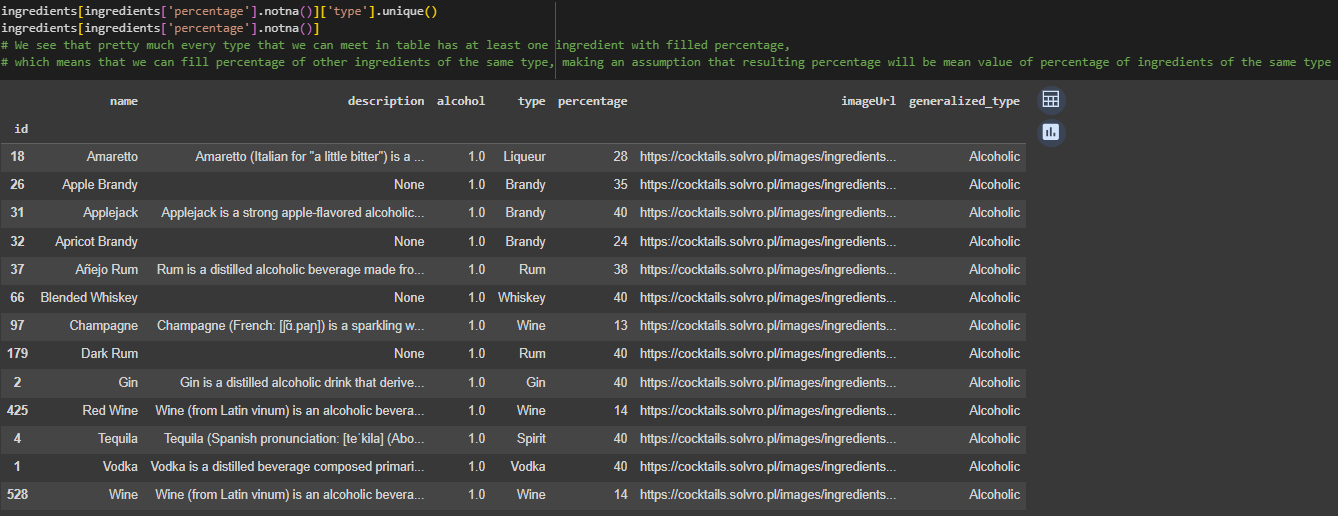
\includegraphics[width=1\linewidth]{ingredients_3.png}
    \caption{Typy alkoholi mające dane o mocności}
\end{figure}

Wcześniej tylko 13 alkoholywch składników mieli dane o mocności, po uzupełnieniu już 44 z 50 wszystkich alkoholowych składników.


\subsection{Tabela koktajli i składników}
Mając osobne tabeli dla koktajli i składników, potrzebujemy jednej któraby ich łączyła. Dlatego z tabeli cocktails która nadal zawiera kolumnę ze składnikami dla koktejla, wyciągamy dane o składnikach do innej tabeli:

\clearpage

\begin{figure}[htbp]
\centering
    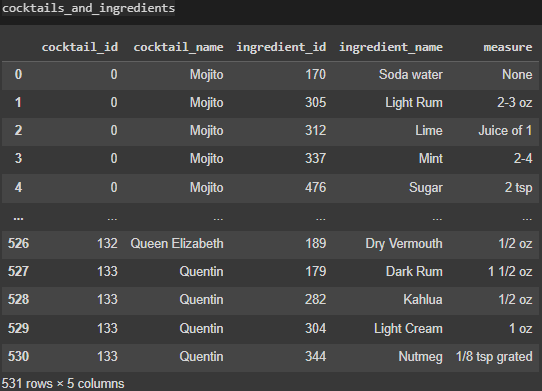
\includegraphics[width=0.6\linewidth]{c_i_1.png}
    \caption{Tabela koktajli i składniki}
\end{figure}

Widać że ona zawiera 531 wiersza i 5 kolumn, z których \textbf{measure} nas najbardziej interesuje.
Spośród wszystkich wierszy tylko 35 nie mają danych o ilości składnika w koktajlu.

\subsubsection{Parsing ilości}

Nas interesują tylko ilości które można skonwertować w uncji(dalej \textbf{oz}), ponieważ tylko oni będą wpływać na mocność koktajla(dalej \textbf{ABV}).
Konwertacji w oz poddają się kolejny ilości:
\begin{itemize}
    \item oz
    \item tblsp - łyżka stołowa
    \item tsp - łyżka herbatna
    \item Juice of - sok (dotyczy limonek i cytryn)
\end{itemize}

\begin{figure}[htbp]
\centering
    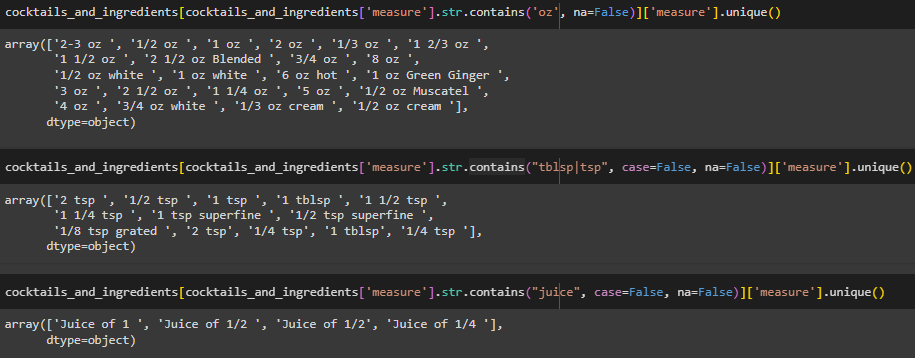
\includegraphics[width=0.6\linewidth]{c_i_2.png}
    \caption{Ilości do parsingu}
\end{figure}


\clearpage

Po parsingu wszystkich ilości możemy zobaczyć wyniki na przykładzie z Mojito, które zawiera składniki ze wszystkimi wymienionymi ilościami oprócz tblsp:

\begin{figure}[htbp]
\centering
    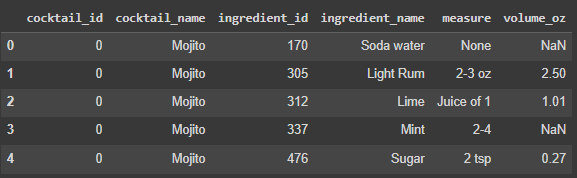
\includegraphics[width=0.7\linewidth]{c_i_3.png}
    \caption{Wynik parsinga}
\end{figure}



\subsection{Tabela koktajli}
\subsubsection{Obliczanie mocności koktajli}

Przed tym jak przejdziemy do obliczania ABV każdego koktajla, zwrócę uwagę na to że na razie to jest możliwe tylko z popełnieniem błędów, albo z pominięciem dużej ilości koktajlów.

\begin{lstlisting}[language=Python]
# For each cocktail, calculate its approximate ABV
for cocktail_id, group in result_df.groupby('cocktail_name'):
    essential_ingrs = []
    for index, row in group.iterrows():

      gen_type = row['generalized_type'] if pd.notna(row['generalized_type']) else "Unknown"
      volume_oz = row['volume_oz']
      percentage = row['percentage']

      if pd.notna(percentage) and pd.notna(volume_oz) and gen_type in ('Alcoholic', 'Non-Alcoholic', 'Fruit'):
        essential_ingrs.append([row['percentage'], row['volume_oz']])

    total_volume, total_alcohol_volume, abv = 0, 0, 0

    for percentage, volume in essential_ingrs:
      total_volume += volume
      total_alcohol_volume += (percentage / 100) * volume

    if total_volume > 0 and total_alcohol_volume > 0:
      abv = (total_alcohol_volume / total_volume) * 100
    else:
      abv = None

    cocktails.loc[cocktails['name'] == cocktail_id, 'abv'] = abv
\end{lstlisting}

Podany kod obliczy ABV dla wszystkich koktajlów które zawierają choćby jeden składnik typu Alcoholic, Non-Alcoholic lub Fruit, który ma dane o jego ilości w oz w tym koktajlu. Takie podejście jest nieprawidłowe i doprowadza do tego że 128 koktajlów będą mieli dane o ABV, ale tylko 54 z nich będą mieli napewno prawdziwe wartości, bo oni nie zawierają składników bez \textbf{generalized-type}. Bo jeżeli koktajl zawiera składnik bez \textbf{generalized-type} i \textbf{volume-oz}, który potencjalnie może być typu \textbf{Non-Alcoholic}, algorytm obliczy ABV bez uwzględnienia tego składniku, co doprowadzi do błędu.
\clearpage
Aby pozbyć się tego problemu, popatrzymy jakie składniki nie mają uogólnienego typu:


\begin{figure}[htbp]
\centering
    \includegraphics[width=0.8\linewidth]{c_i_4.png}
    \caption{Składniki bez generalized-type}
\end{figure}

Takich które owszem wpływają na ABV koktajlu jest niedużo, mianowice:
\begin{itemize}
    \item Benedictine - jest mocnym likierem
    \item Bitters - rodzina mocnych likierów
    \item Club Soda
    \item Lemon vodka
    \item Soda water
\end{itemize}

I od razu na miejscu naprawimy te typy które nie uwzględnił mapper w punkcie 3.1.1.

Znów powtarzamy obliczenie ABV, ale już innym algorytmem który uwzględnia brak danych o ilości składnika który jest typu Alcoholic, Non-Alcoholic. Teraz już 68 koktajli mają dane o mocności, co oznacza że naprawienie typów niektórych składników i zmiana algorytmu uratowali nam dane o mocności 14 koktajli.

\begin{figure}[htbp]
\centering
    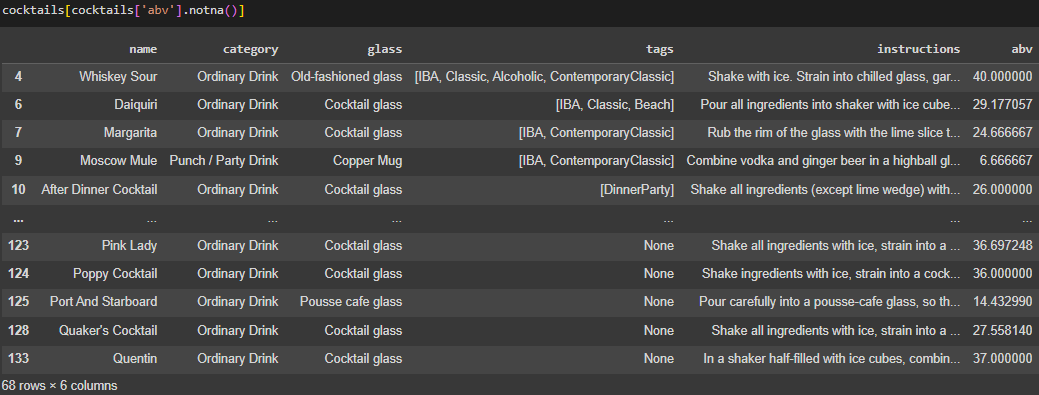
\includegraphics[width=0.8\linewidth]{c_i_5.png}
    \caption{Koktajli z danymi o ABV}
\end{figure}

\subsubsection{Kategorię mocności koktajli}

Pod koniec rozdzielimy koktajli na kategorię według ich mocności:
\begin{itemize}
    \item ABV is \texttt{na} - Unknown
    \item ABV $<$ 10\% - Weak
    \item 10\% $\leq$ ABV $<$ 20\% - Moderate
    \item 20\% $\leq$ ABV $<$ 30\% - Strong
    \item ABV $\geq$ 30\% - Very Strong
\end{itemize}

\subsubsection{Długość instrukcji, liczba składników, sposób przyrządzenia}
Dla przyszłej analizy dodamy kolumnę z długością instrukcji, liczbą składników w koktajlach i ich sposobem przyrzadzenia(ekstraktowany z instrukcji):
\begin{figure}[htbp]
\centering
    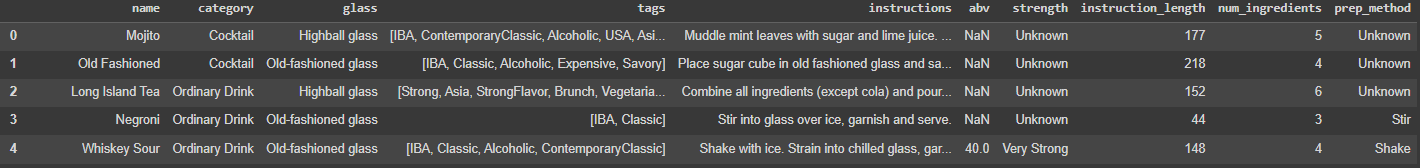
\includegraphics[width=1\linewidth]{cocktails_2.png}
    \caption{Koktajli z nowymi kolumnami}
\end{figure}


\section{Ewaluacja}
W tym punkcie będą załączone wszelkie wykresy pokazujący charakter naszych danych.
\subsection{Koktajli}
\begin{figure}[ht]
    \centering
    \begin{subfigure}{0.45\textwidth}
        \centering
        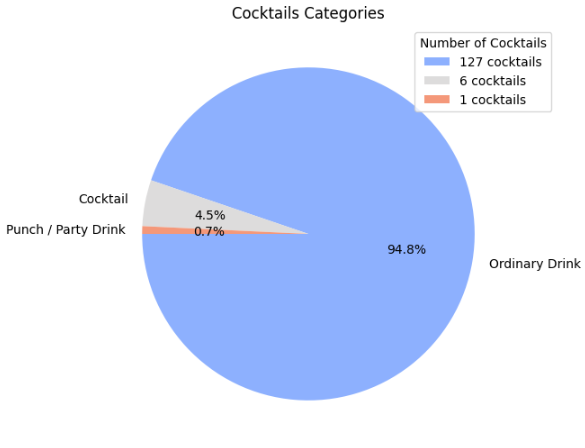
\includegraphics[width=\textwidth]{c_p_1.png}
        \label{fig:image1}
    \end{subfigure}
    \hfill
    \begin{subfigure}{0.38\textwidth}
        \centering
        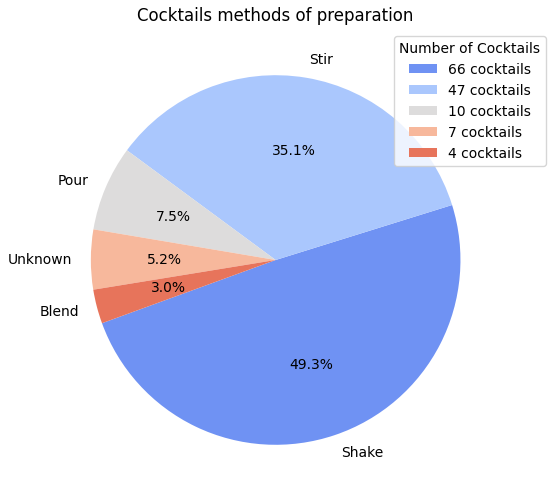
\includegraphics[width=\textwidth]{c_p_2.png}
        \label{fig:image2}
    \end{subfigure}
    \caption{Jak widać prawie wszystkie koktajli są Ordinary Drinka'ami, i prawie połowe koktajli trzeba mieszać w szejkerze.}
\end{figure}

\begin{figure}[h]
\centering
    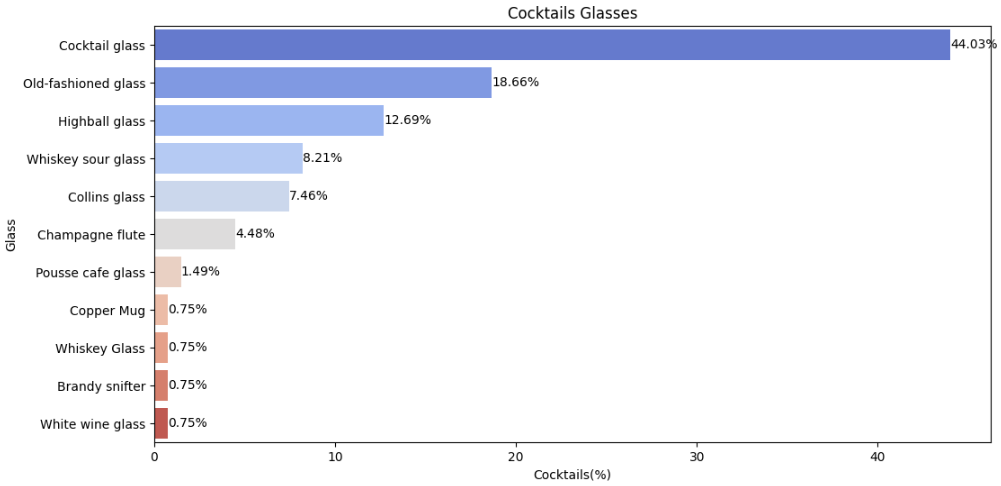
\includegraphics[width=1\linewidth]{c_p_3.png}
    \vspace{2cm}
    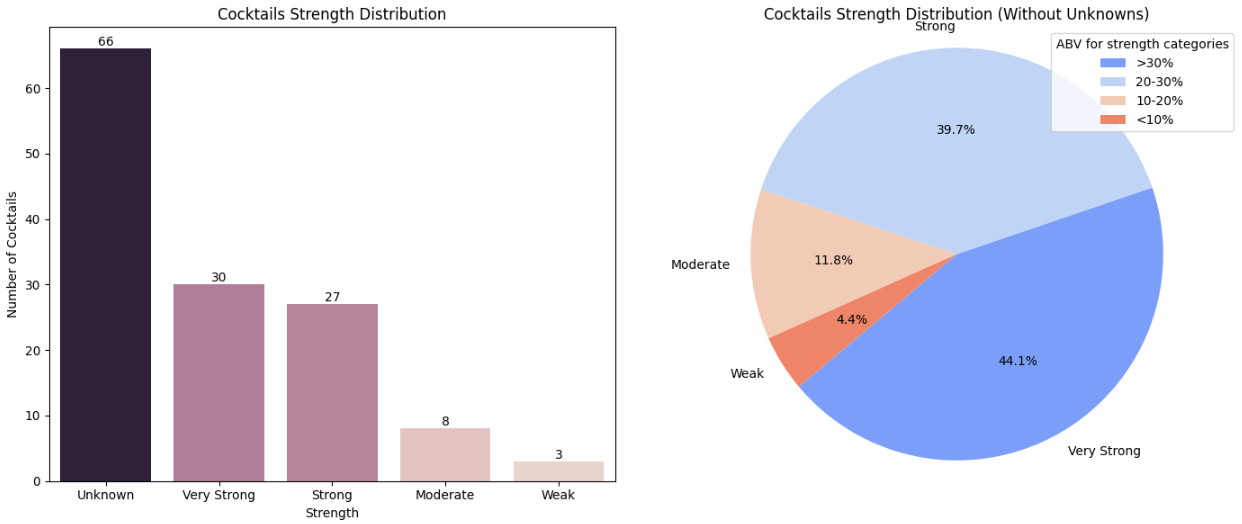
\includegraphics[width=1\linewidth]{c_p_8.png}
    \caption{Większość koktejli jest nalewana w szklankę koktajlową, a aż 85\% koktajlów jest mocniej 20\%.}
\end{figure}

\clearpage

\subsection{Składniki}

\begin{figure}[h]
\centering
    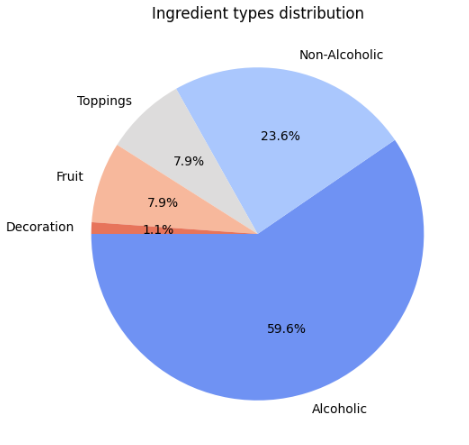
\includegraphics[width=0.45\linewidth]{i_p_1.png}
    \vspace{2cm}
    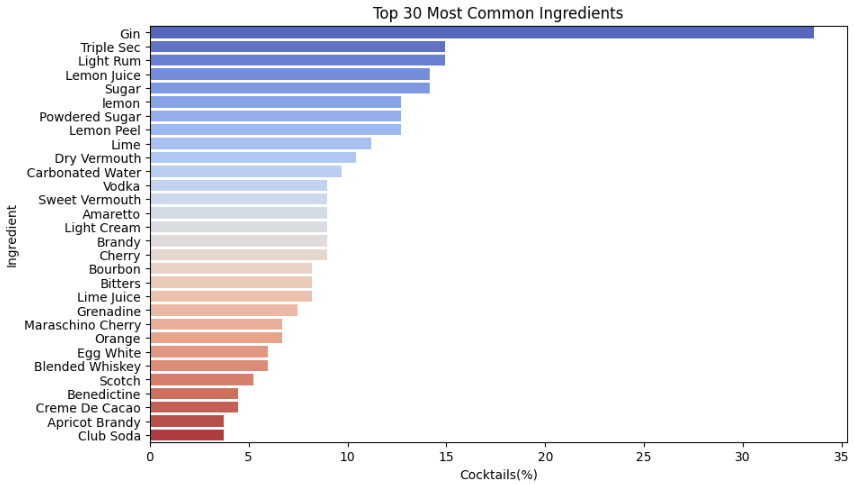
\includegraphics[width=0.7\linewidth]{i_p_2.png}
    \caption{Widzimy że ponad połowa składników jest alkoholowa, z których Gin jest wykorzystywany najczęściej. A sok cytryny jak widać jest jednym z najpopularniejszych składników.}
\end{figure}

\begin{figure}[h]
\centering
    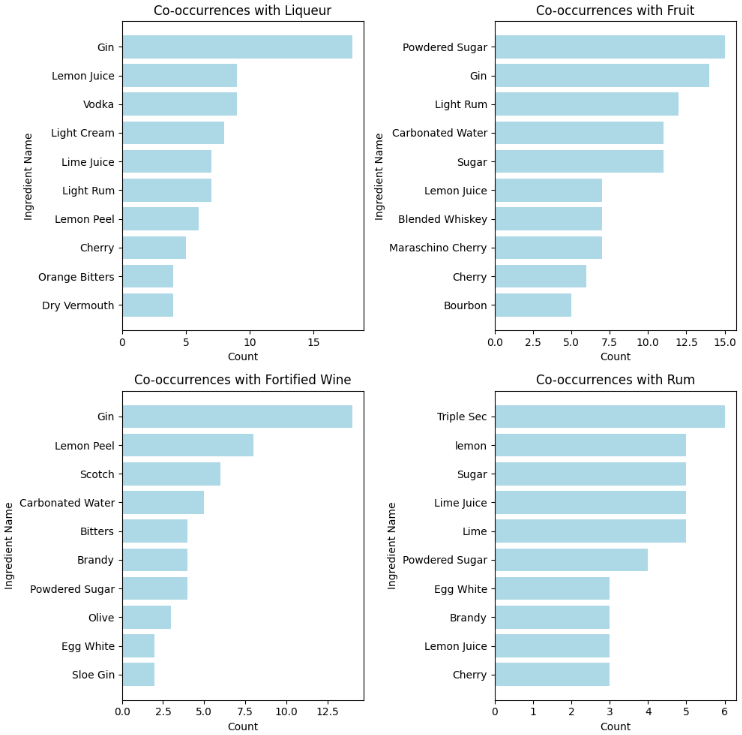
\includegraphics[width=0.6\linewidth]{i_p_3.png}
    \vspace{2cm}
    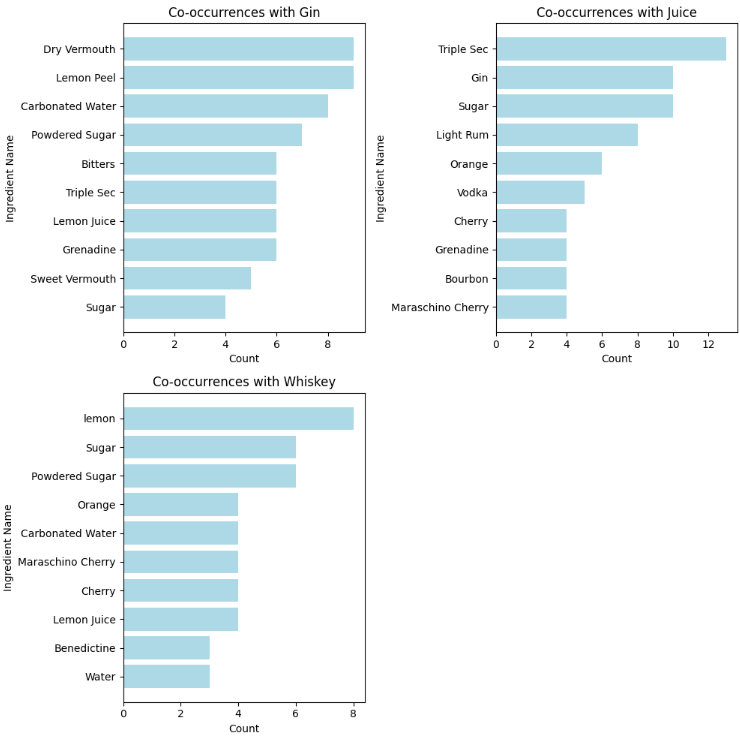
\includegraphics[width=0.6\linewidth]{i_p_4.png}
    \caption{Widzimy że najpopularniejszy gin zazwyczaj razem nie występuje tylko z romem i whisky. Ale widać że gin często jest razem z vermutem - jak jeszcze przyrządzić wszelkie martini? Likiery często pijemy z sokiem cytryny. A do owoców często dodajemy cukier. Whiski często serwujemy z cytryną(z sokiem rzadziej). Natomiast rom też serwowany z cytryną lub limonką, zazwyczaj pijemy z sokiem limonki a nie cytryny.}
\end{figure}


\clearpage

\subsection{Koktajli i składniki}
\begin{figure}[ht]
    \centering
    \begin{subfigure}{0.45\textwidth}
        \centering
        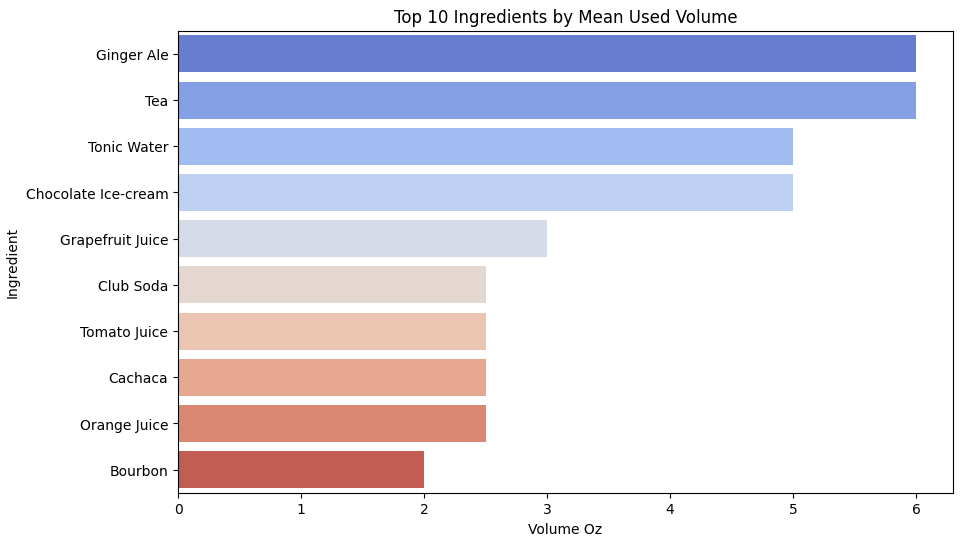
\includegraphics[width=\textwidth]{c_i_p_1.png}
        \label{fig:image1}
        \caption{Mocno rozwadniamy wódkę w Moscow Mule ginger ale'em, i herbatą Amaretto Tea - deserowy koktajl.}
    \end{subfigure}
    \hfill
    \begin{subfigure}{0.45\textwidth}
        \centering
        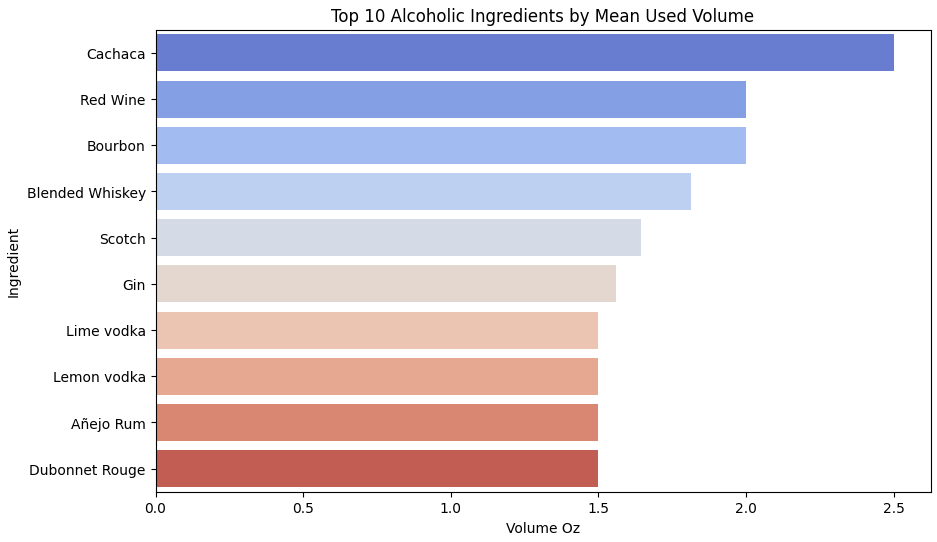
\includegraphics[width=\textwidth]{c_i_p_2.png}
        \label{fig:image2}
        \caption{Robimy mocne koktajli z cachaca i bourbonem, i trochę mniej mocne z ginem i wódkami.}
    \end{subfigure}
    
\end{figure}

\begin{figure}[h]
\centering
    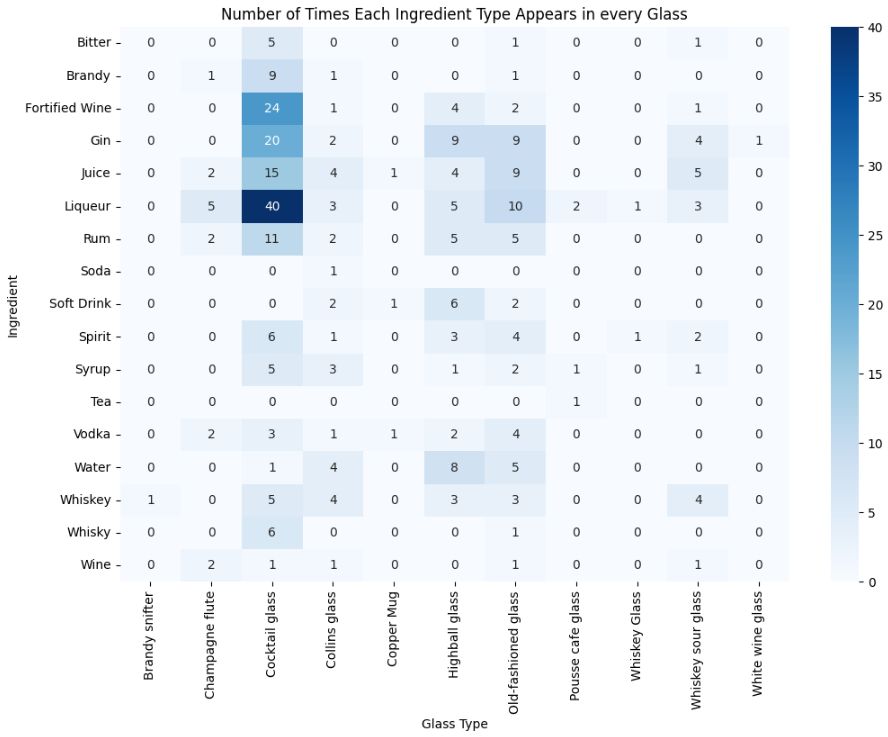
\includegraphics[width=0.7\linewidth]{c_i_p_3.png}
    \caption{Jak widać, większość koktajlów jest nalewana szklankę koktajlową - w tym najwięcej koktajlów na podtsawie likierów i wzmocnionych win i gina. Widać że sporo składników jest stosowana w koktajlach w old-fashioned glass.}
\end{figure}


\begin{figure}[h]
\centering
    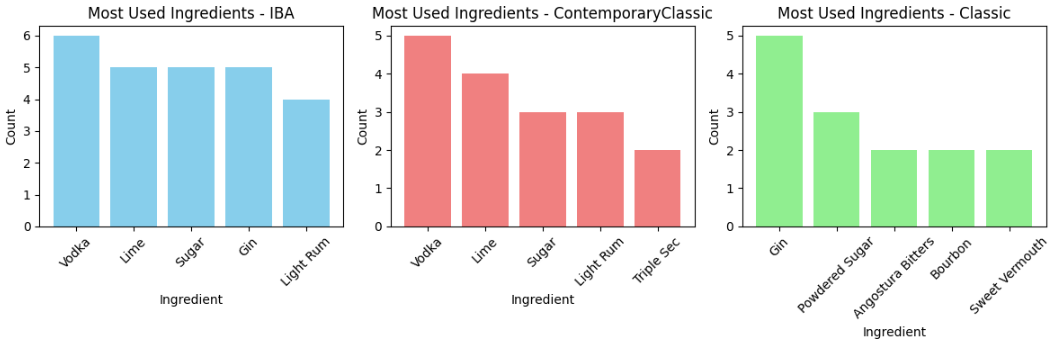
\includegraphics[width=1\linewidth]{c_i_p_4.png}
    \caption{Widzimy, że klasyczne koktajle są zwykle robione z Ginem (Martini itp.), podczas gdy współczesna Klasyka bardziej koncentruje się na wódce z limonką. A koktajle IBA powstają głównie z wódki i ginu.}
    \vspace{2cm}
    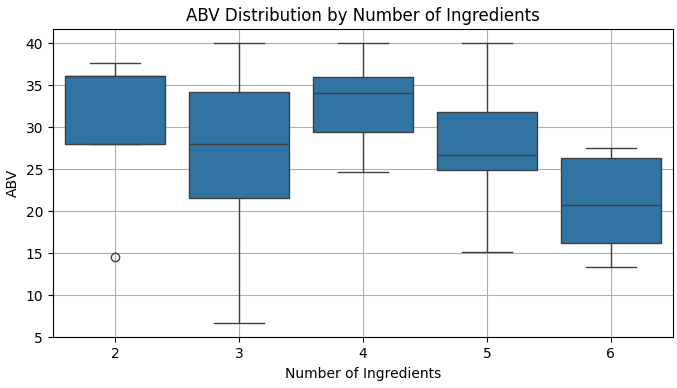
\includegraphics[width=0.8\linewidth]{c_i_p_5.png}
    \caption{Na tym wykresie widać trend na spadek mocności koktajlów przy zwiększeniu liczby składników. Serwując tylko dwa składniki - chcemy posmakować ich kombinację bez rozwodnienia. Serwując 6 - szukamy nowych smaków na podstawie alkoholowych składników.}
\end{figure}

\clearpage

\section{Ciekawostka}
Jeżeli nie chcemy wydawać pieniędzy na wycieczkę do baru, aby spróbować ciekawe kombinacji składników odnalezione podczas analizy - możemy kupić kilka składników i przyrządzić koktajlę w domu. Ale które składniki warto kupić jeżeli chcemy przyrządzić jak najwięcej koktajlów?

\textbf{optimizer.py} zawiera rozwiązanie tego zadania liniowego programowania, które pomoże określić te \textbf{n} składników za pomocą których potrafimy spróbować jak najwięcej koktajlów.
Optimizer posiada możliwość rozwiązania tego zadania na dwa sposoby:
\begin{itemize}
    \item Odnalezienie \textbf{n} składników za pomocą których będzie można przyrządzić największą liczbę koktajli
    \item Odnalezienie \textbf{n} alkoholowych składników na podstawie których, z dodaniem reszty nie alkoholowych składników, można przygotować jak najwięcej koktajli
\end{itemize}

Drugi punkt brzmi ciekawiej, bo zakupienie alkoholowych składników jest dość drogie, co oznacza że nie potrafimy dużo ich kupić, a nie alkoholowe: wszelkie soki, owoce i toniki nie są aż tak drogie, i ich już można kupić dość dużo i przyrządzić tym więcej koktajlów.

Przykład działania:
\begin{figure}[ht]
    \centering
    \begin{subfigure}{0.45\textwidth}
        \centering
        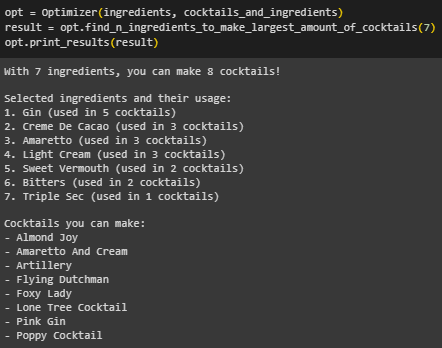
\includegraphics[width=\textwidth]{opt_1.png}
        \label{fig:image1}
        \caption{Te koktajli raczej będą dość podobne do siebie.}
    \end{subfigure}
    \hfill
    \begin{subfigure}{0.38\textwidth}
        \centering
        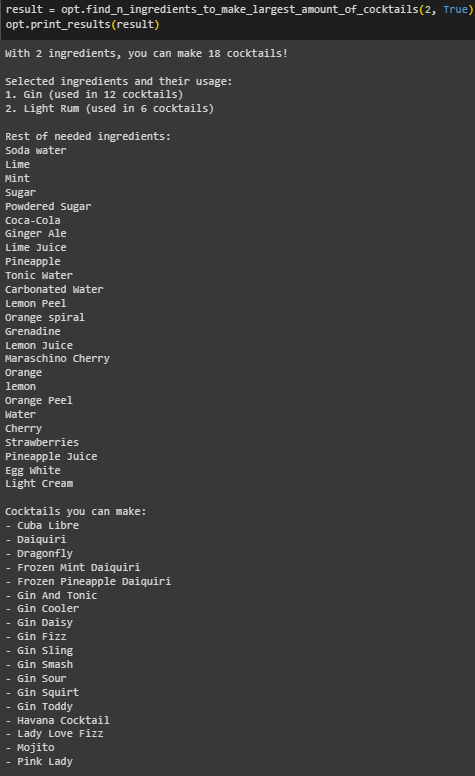
\includegraphics[width=\textwidth]{opt_2.png}
        \label{fig:image2}
        \caption{Nawet z 2 alkoholi można przyrządzić sporo koktajli, chociaż też dość podobnych. Warto wtedy kupić jeszcze choćby 2 innych alkohola.}
    \end{subfigure}
    
\end{figure}

\clearpage

\section{Klasteryzacja}
Głównym celem klasteryzacji koktajli oczywiście jest zgrupowanie ich tak, aby w każdej grupie byli koktajli najbardziej podobne do siebie.
\newline
Najsensowniej określać podobieństwo koktajli w zależności od ich składników, od tego i zaczniemy.
\subsection{Klasteryzacja na podstawie składników}
Klasteryzować będziemy na podstawie objętości składników w koktajlach, jeżeli nie mamy danych o objętośi w oz pewnych składników w koktajlu, zamieniamy ich na 0.01 oz, nie najlepsze podejście, ale działa dla wszystkich składników, nawet dla wszelkich jagod i owoców stosowanych dla dekaracji koktajli.

\newline

Zaczniemy od klasteryzacji za pomocą KMeans z \textbf{n\_clusters=5}, bo tyle jest podstawowych smaków - salty, spicy, sweet, sour, bitter - jest to naiwnie wierzyć że KMeans rozdzieli koktajli akkurat według smaków, ale niech będzie 5.
\begin{figure}[h]
\centering
    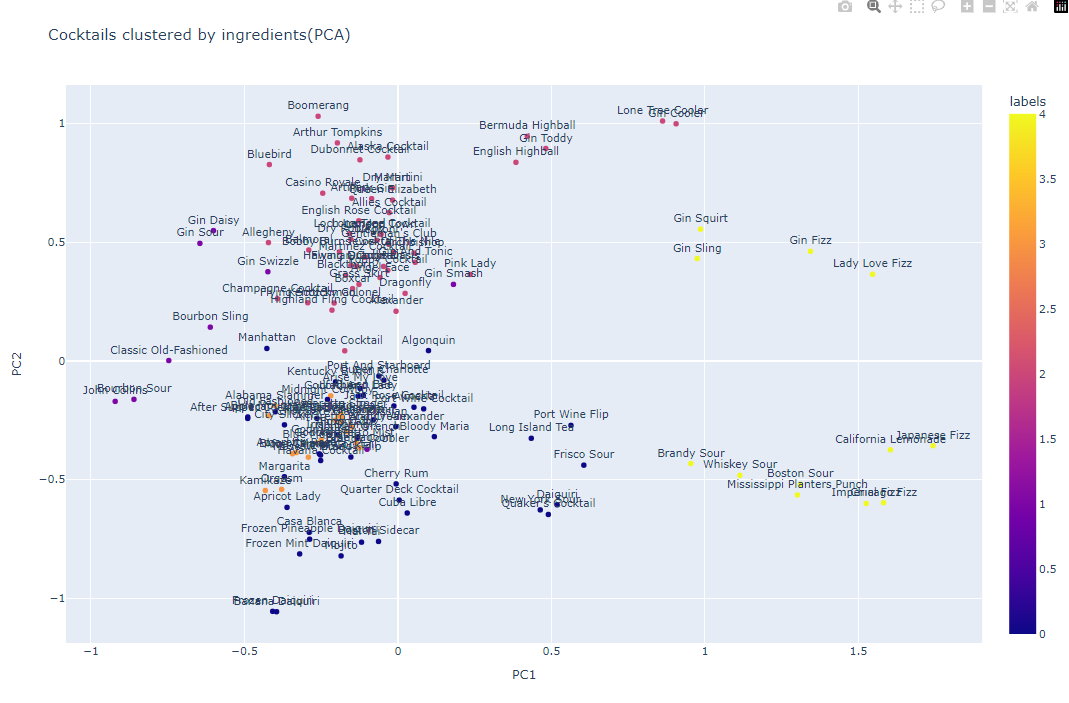
\includegraphics[width=1\linewidth]{cluster_1.png}
    \caption{Wizualizacja koktajli za pomocą PCA.}
\end{figure}

Na wykresie widzimy sporo tłumu który bez przybliżenia nie pozwala nawet odczytać nazw koktajlów, ale nawet jeżeli przybliżmy ten wykres, zauważymy że często jest tak że koktajli które są blisko siebie, mogą nawet nie mieć wspólnych składników, co oznacza że PCA nie potrafił dobrze zwizualizować koktajle na 2D wykresie - sprawdzimy dlaczego.

\clearpage

\begin{figure}[h]
\centering
    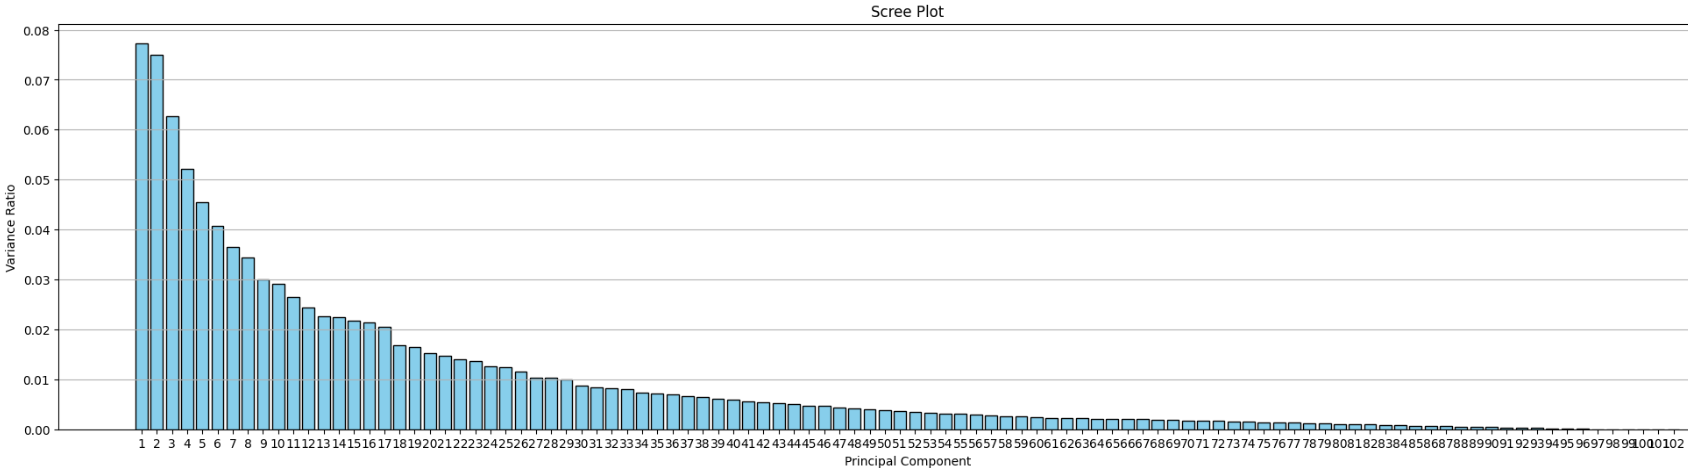
\includegraphics[width=1\linewidth]{cluster_2.png}
    \caption{Wariancja principal components.}
\end{figure}

Na tym wykresie widzimy poziomy wariancji wszystkich PC dla naszego PCA. Widać że PC1 i PC2 w sumie odpowiadają tylko za około 16.5\% od całej wariancji, co jest za mało dla wizualizacji koktajli na 2D wykresie. Dlatego spróbójmy zastosować inną metodę do wizualizacji.

\begin{figure}[h]
\centering
    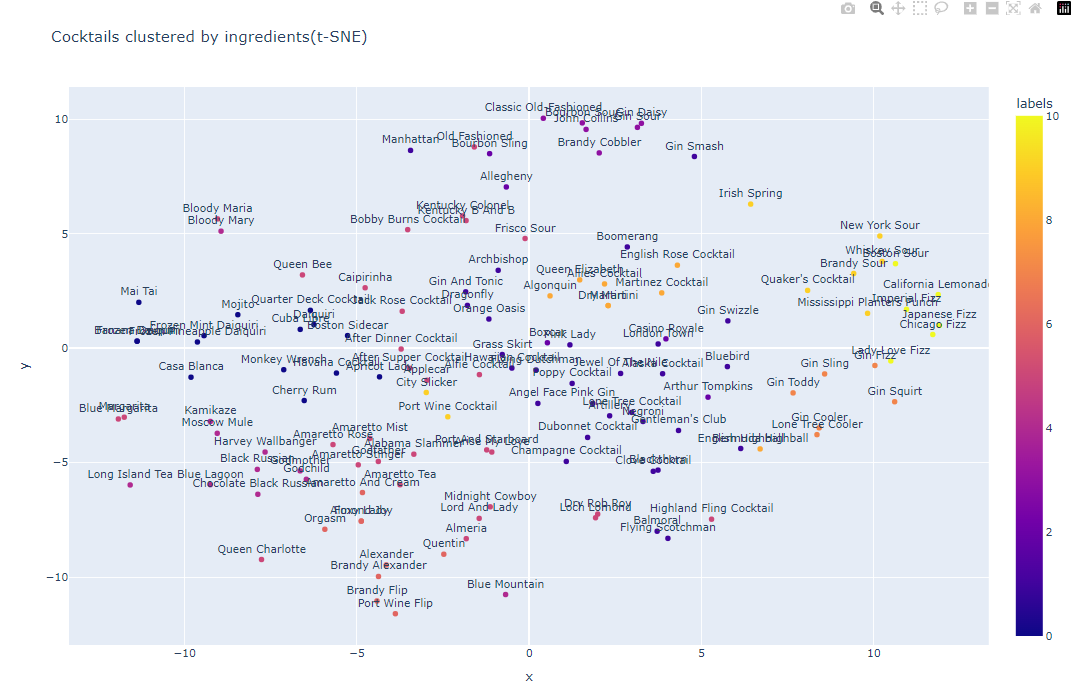
\includegraphics[width=1\linewidth]{cluster_3.png}
    \caption{Wizualizacja koktajli za pomocą t-SNE.}
\end{figure}

Wizualizacja za pomocą bardziej współczesnej metody t-SNE już wygląda o wiele lepiej i nawet jeżeli sprawdzimy składniki koktajli leżących blisko siebie, zauważymy że owszem składniki są podobne! 
\newline
Jedyna ciekawostka jest w tym, że ten wykres może nieść w sobie jeszcze więcej informacji, bo na razie kolory koktajlów tak naprawdę określają grupy koktajli najbardziej do siebie podobnych, co jest przydatne dla stworzenia pewnego spisu koktajli z rozdzieleniem na grupy według klasterów, ale nic więcej nam nie mówią, i możemy spróbować to zmienić.

\clearpage

\begin{figure}[h]
\centering
    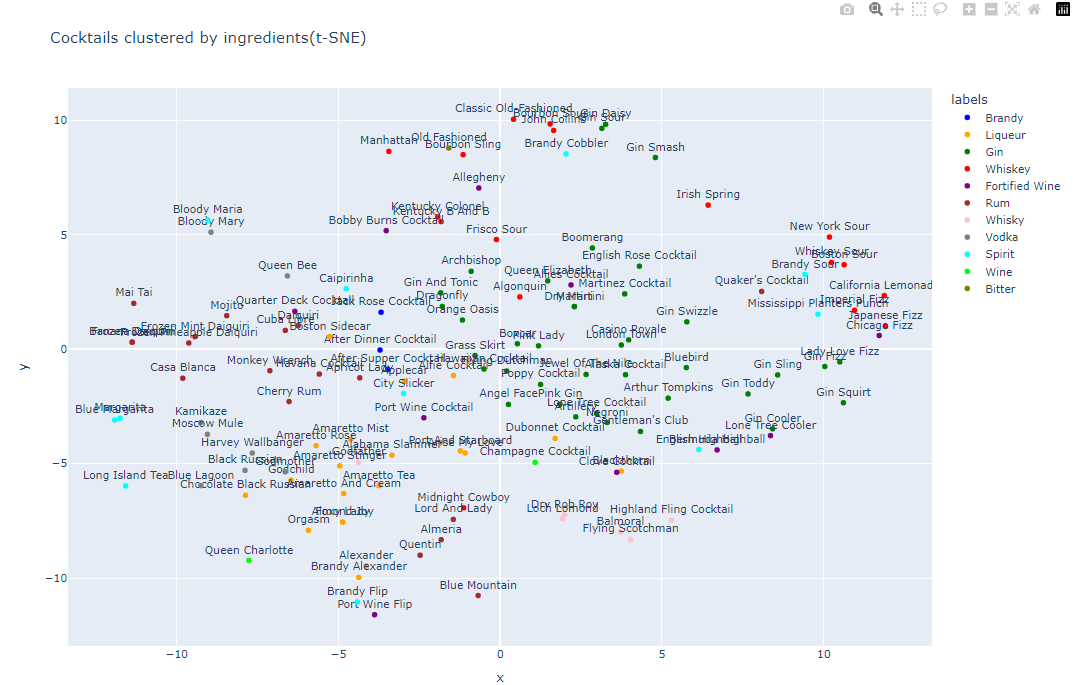
\includegraphics[width=1\linewidth]{cluster_4.png}
    \caption{Wizualizacja koktajli za pomocą t-SNE i kolorowanie na podstawie typu głownego alkoholu.}
\end{figure}


Ten wykres jest jeszcze lepszy od zeszłego, ponieważ teraz kolory mają sens i poza tym nawet widać że zazwyczaj koktajli o tej samej podstawie alkoholowej są blisko siebie, chociaż takie podejście nadal nie jest idealne, bo czasami koktajli mają kilka alkoholowych składników o tej samej objętości i ich głowny jest wybierany "losowo" spośród tych.

\clearpage

\subsection{Klasteryzacja na podstawie "stylu" przyrządzenia}
Oprócz składników możemy również klasteryzować nasze koktajle na podstawie innych parametrów m.in:

\begin{itemize}
    \item Glass
    \item Strength
    \item Num ingredients
    \item Preparation method
\end{itemize}

Dla stosowania \textbf{Glass} i \textbf{Preparation method} w klasteryzacji i wizualizacji musimy przekształcić ich do liczbowej postaci - zrobimy to za pomocą \textbf{OneHotEncoder}.

\begin{figure}[h]
\centering
    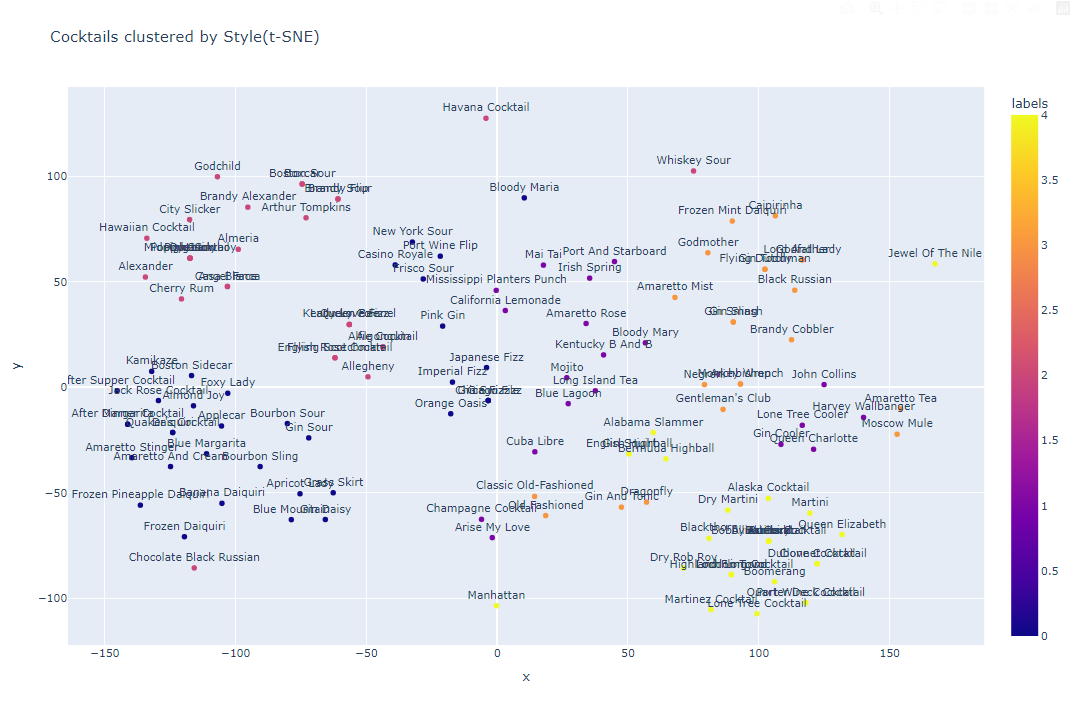
\includegraphics[width=1\linewidth]{cluster_8.png}
    \caption{Wizualizacja koktajli za pomocą t-SNE i kolorowanie na podstawie KMeans.}
\end{figure}

Jeżeli porównać koktajli leżące blisko siebie, zauważymy że zazwyczaj są podobnej mocności, przyrządzane tym samym sposobem i mają mniej więcej tyle same składników, ale już rzadziej są nalewane w te same szklanki.

\clearpage

Z ciekawości pomalujemy koktajle na tym wykresie na podstawie typu ich głównego alkoholego składniku.

\begin{figure}[h]
\centering
    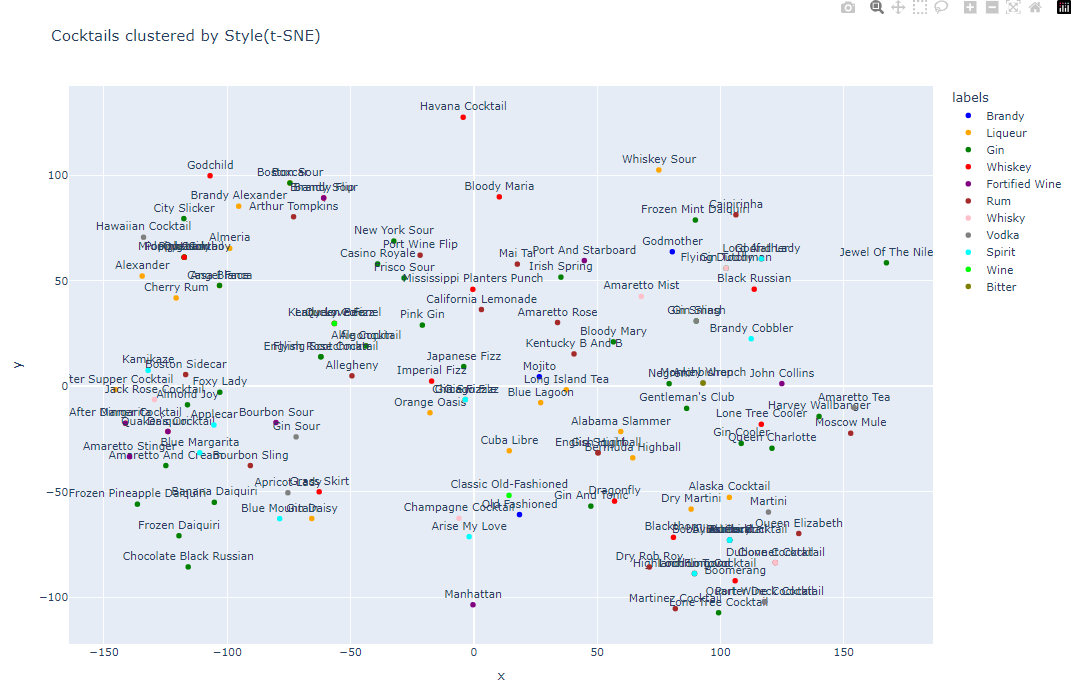
\includegraphics[width=1\linewidth]{cluster_7.png}
    \caption{Wizualizacja koktajli za pomocą t-SNE i kolorowanie na podstawie typu głównego składniku.}
\end{figure}


Widać że koktajle o tych samych kolorach prawie nie formują klastery, z czego wynika że "styl" koktajlu nie bardzo zależy od jego głównego składniku.


\section{Wnioski}
Podczas tej analizy zauważyliśmy sporo zależności między różnymi danymi o koktajlach, ale najcenniejszymi są:
\begin{itemize}
    \item Gin jest najpopularniejszym składnikom koktajli.
    \item ABV koktajlów zazwyczaj spada przy zwiększeniu liczby składników.
    \item Nawet z niedużej ilości różnych alkoholi można przyrządzić wiele koktajlów.
    \item Da się klasteryzować koktajli i nawet w na tyle dobry sposób, że z tego można korzystać w praktyce.
\end{itemize}



\end{document}
